% RF coupling
\chapter{RF Coupling}
\label{chap:rf_coupling}
%\margintoc
This chapter aims to give the key elements in order to derive the optimum characteristics for RF plasma heating or current drive antennas. The section \ref{sec:waves-in-plasma} first characterizes the propagation medium, in particular the kind of modes that can propagate in the plasma as a response to a given excitation. The sections \ref{sec:icrh} and \ref{sec:lhcd} focuses on the specific range of frequencies of ICRF and LHCD. 

Many antenna-plasma coupling models have been developed and most rely on a "slab" approximation which consists in assuming uniformity in the toroidal and poloidal directions while imposing a radiation boundary condition in the radial direction. While much of the essential physics of the coupling at the plasma–antenna interface can be elucidated using this slab approximation, real-life experiments presents additional problems since plasma is not homogeneous, antenna geometries can be complex, images currents are induced on the passive conducting elements surrounding the antenna and wave excitation not perfect. Thus, plasma response and wave fields must be solved with more refinements, treating the antenna geometry as accurately as possible. Antenna-plasma coupling is still a topic of continued research interest and some contributions are presented in Section~\ref{sec:ALOHA}, \ref{sec:LHCD_FW_antena_coupling} and \ref{sec:ICRH_FW_antena_coupling}.


\section{RF Waves In Plasma}\label{sec:waves-in-plasma}
This section is a reminder of the basic properties of wave propagation in a magnetized plasma. In-depth treatment and derivations of the results given in this section can be found in the standards physics oriented textbooks \sidecite{stix1992, Brambilla1998, Swanson2003, Cairns1991, Golant1989}. 

\subsection{Maxwell Equations in Time Harmonic Regime}
We shall start the Maxwell equations is their most general form, before recasting them to fit our needs. The usual electromagnetic field quantities are expressed in terms of six quantities that are, following the terminology used \sidecite{Harrington2001}:
\begin{itemize}
	\item $\boldsymbol{\mathcal{E}}$: the electric field intensity (in $\si{V/m}$)
	\item $\boldsymbol{\mathcal{H}}$: the magnetic field intensity (in $\si{A/m}$)
	\item $\boldsymbol{\mathcal{D}}$: the electric flux density (in $\si{A.s/m^2=C/m^2}$)
	\item $\boldsymbol{\mathcal{B}}$: the magnetic flux density (in $\si{V.s/m^2=Wb/m^2}$, also known as Tesla $\si{T}$)
	\item $\boldsymbol{\mathcal{J}}$: the electric current density (in $\si{A/m^2}$)
	\item $q_v$: the electric charge density (in $\si{C/m^3}$)
\end{itemize}
where all quantities are function of space and time, e.g. $\boldsymbol{\mathcal{E}}=\boldsymbol{\mathcal{E}}(\mathbf{r},t)$. 

Maxwell equations can be stated as:
\begin{subequations}
	\begin{align}
		\boldsymbol{\nabla} \times \boldsymbol{\mathcal{E}} &= -\frac{\partial \boldsymbol{\mathcal{B}}}{\partial t} \label{eq:Maxwell-Faraday}\\
		\boldsymbol{\nabla} \times \boldsymbol{\mathcal{H}} &= \frac{\partial \boldsymbol{\mathcal{D}}}{\partial t} + \boldsymbol{\mathcal{J}} \label{eq:Maxwell-Ampere} \\
		\boldsymbol{\nabla} \cdot \boldsymbol{\mathcal{D}} &= q_v \label{eq:Maxwell-Gauss} \\
		\boldsymbol{\nabla} \cdot \boldsymbol{\mathcal{B}} &= 0 \label{eq:Maxwell-Gauss-Magnetism}
	\end{align}
	\label{eq:MaxwellEquations}
\end{subequations} 
with $\mu_0=4\pi\times10^7~\si{H/m}$ the vacuum magnetic permeability and $\varepsilon_0=1/(\mu_0 c^2)~\si{F/m}$ the vacuum dielectric permittivity with $c$ the speed of light.

The previous expressions are non-linear by nature. We will limit our analysis to a stationary and an homogeneous plasma. Moreover, we will assume that Radio-Frequency source time excitation varies sinusoidally in time with a single frequency. Such case of time varying electromagnetic fields is referred as time-harmonic  \sidecite{Harrington2001} and the analysis of fields quantities $\boldsymbol{\mathcal{A}}$ can be simplified by using complex quantities $\Abf$\footnote{The choice of the time sign convention $+j\omega t$ is motivated to match the one adopted in most RF solvers, commercial or the ones developed in this work, which is most prevalent in electrical engineering texts. Note that in general, waves in plasma texts use the opposite sign convention, ie. $e^{-i\omega t}$\cite{bradley2007, michelsen2019}. While both conventions are mathematically valid, the use of $exp(–j\omega t)$ can be preferable when dealing with the principal value of complex number square roots, which does not require numerical tricks as the ones defined for example in \cite{Hillairet2007a}. Using $j=-i$ allows one to convert results from one convention to the other.}:
\marginnote{We will adopt $j$ as the complex unit, ie. $j^2=-1$.}
\begin{equation}
\boldsymbol{\mathcal{A}}(\rbf,t) 
	\stackrel{\Delta}{=} 
	\left| \Abf(\rbf) \right| \cos\left(\omega t + \phi \right) 
	= 
	\Re \left[ \Abf(\rbf) e^{j\omega t} \right]
\end{equation}
\marginnote{This solution can be generalized to finite bandwidth cases, which are a continuous distribution of frequencies $\omega$, by defining the field as summation of time-harmonic solutions over all frequencies: 
$$
\boldsymbol{\mathcal{A}}(\rbf,t) 
	\stackrel{\Delta}{=} 
	 \int \diff \omega \Re\left[\boldsymbol{\mathcal{A}}(\rbf,\omega)e^{j\omega t}  \right]
$$
which can be seen as a time-domain Fourier transform. Moreover, since $\boldsymbol{\mathcal{A}}(\rbf,t) $ is real function, then $\boldsymbol{\mathcal{A}}(\rbf,-\omega)=\boldsymbol{\mathcal{A}}^*(\rbf,\omega)$ by property of the Fourier transform.}

It is also convenient to represent field phasors $\Abf(\mathbf{r})$ in the Fourier space using plane-wave expansion \sidecite[+5cm]{clemmow1996}: 
\begin{equation}
		\boldsymbol{\mathcal{A}}(\mathbf{r}, t) 
		=
		\Re \left[
		\int \diff \kbf \;
		\mathbf{A}(\kbf) e^{j(\omega t - \kbf\cdot\rbf)}
		\right]
	\label{eq:k-spectralDefinition}
\end{equation}
where each plane wave is characterized by their wavevector $\kbf=(k_x, k_y, k_z)$. 

Plugging such a solution into the Maxwell equations (\ref{eq:MaxwellEquations}) leads to algebraic equations:
\begin{subequations}
	\begin{align}
		\kbf \times \Ebf (\kbf) 
		=& 
		\omega \Bbf (\kbf)
		\\
		\kbf \times \Hbf (\kbf) 
		=& 
		-\omega \Dbf (\kbf)
		+ 	
		j\Jbf (\kbf) 
		\\
		\kbf  \cdot \Dbf (\kbf) 
		=& j q_v(\kbf) 
		\\
		\kbf  \cdot \Bbf (\kbf) 
		=& 0
	\end{align}
	\label{eq:k-omegaMaxwellEquations}
\end{subequations}

% ###########################################################################
% ###########################################################################
\subsection{Constitutive Relations}
Fluxes densities $(\boldsymbol{\mathcal{D}}, \boldsymbol{\mathcal{B}})$ differ from field intensities $(\boldsymbol{\mathcal{E}}, \boldsymbol{\mathcal{H}})$ inside materials with regards to their relative magnitude and direction. Flux densities can be interpreted  as a response of the medium to an applied excitation. One can thus express $(\boldsymbol{\mathcal{D}},\boldsymbol{\mathcal{B}})$ and $\boldsymbol{\mathcal{J}}$ in terms of $(\boldsymbol{\mathcal{E}},\boldsymbol{\mathcal{H}})$, also known as the constitutive relationships written in the most general form as\sidecite{Harrington2001}:
\begin{subequations}
	\begin{align}
		\boldsymbol{\mathcal{D}} =& \boldsymbol{\mathcal{D}}(\boldsymbol{\mathcal{E}},\boldsymbol{\mathcal{H}}) \\
		\boldsymbol{\mathcal{B}} =& \boldsymbol{\mathcal{B}}(\boldsymbol{\mathcal{E}},\boldsymbol{\mathcal{H}}) \\
		\boldsymbol{\mathcal{J}} =& \boldsymbol{\mathcal{J}}(\boldsymbol{\mathcal{E}},\boldsymbol{\mathcal{H}})
	\end{align}
\end{subequations}
Some situations may arise where the induction fields are no more linearly proportional to the primitive intensity fields. In such cases, one needs to extend the definition of linearity using linear differential relations\sidecite{Mackay2010}:
\begin{subequations}
	\begin{align}
		\boldsymbol{\mathcal{D}} &= \varepsilon \boldsymbol{\mathcal{E}} + \varepsilon_1 \boldsymbol{\mathcal{E}}^2  + \ldots \\
		\boldsymbol{\mathcal{B}} &= \varepsilon \boldsymbol{\mathcal{H}} + \varepsilon_1 \boldsymbol{\mathcal{H}}^2 + \ldots \\
	\end{align}
\end{subequations}
Such situation arises typically when high intensity RF fields are used, which leads to non-linear phenomenons such \emph{ponderomotive effect}\sidecite{Krapchev1979}, an effect studied for LHCD in \sidecite{preynas2013}.



Appendix TODO shows that a magnetized plasma can be considered as an anisotropic medium for electromagnetic waves.  In such case, the response of the medium is different depending on the direction of the oscillating field and expressed by tensor constitutive relationships. Since we have assumed that the plasma is homogeneous and stationnary, constitutive relations become algebraic time-invariant relationships\sidecite{Dumont2017}%\marginnote{We will admit the generalized Ohm's law $\Jbf(\Ebf)=\sigma\Ebf$.}:
\begin{subequations}
	\begin{align}
		\Dbf(\kbf, \omega) 
		=& 
		\boldsymbol{\varepsilon}(\kbf, \omega) \cdot \Ebf(\kbf, \omega) 
		\label{eq:disp_relation_kw_D}
		\\
		\Bbf(\kbf, \omega) 
		=& 
		\boldsymbol{\mu}(\kbf, \omega) \cdot \Hbf(\kbf, \omega) 
		\label{eq:disp_relation_kw_B}
		\\
		\Jbf(\kbf, \omega) 
		=& 
		\boldsymbol{\sigma}(\kbf, \omega) \cdot \Ebf(\kbf, \omega) 
		\label{eq:disp_relation_kw_J}
	\end{align}
	\label{eq:k-omegaDispersionRelation}
\end{subequations}
where $\boldsymbol{\varepsilon}$, $\boldsymbol{\mu}$ and $\boldsymbol{\sigma}$ are the dielectric tensor, the permeability tensor and the conductivity tensor respectively, which can be interpreted as 3x3 matrices\sidecite{Swanson2003}. Maxwell equations (\ref{eq:k-omegaMaxwellEquations}) reads with the supplementary assumption that the medium is non magnetic (i.e. $\boldsymbol{\mu}=\mu_0$):\marginnote{The $(\kbf,\omega)$ dependance is assumed from now for the ease of reading.}
\begin{subequations}
	\begin{align}
		\kbf \times \Ebf  
		=& 
		\omega \mu_0 \Hbf
		\\
		\kbf \times \Hbf 
		=& 
		\left(
		-\omega \boldsymbol{\varepsilon} 
		+ 	
		j\boldsymbol{\sigma} 
		\right) \cdot 
		\Ebf
		\\
		\kbf  \cdot \boldsymbol{\varepsilon}  \cdot \Ebf 
		=& jq_v
		\\
		\kbf  \cdot \Hbf 
		=& 0	
	\end{align}
\end{subequations}

Combining the first two equations leads to the wave equation:
\begin{equation}
\nbf \times \nbf \times \Ebf + \Kbf \cdot \Ebf = 0
\end{equation}
where $\nbf = \kbf / \norm{\kbf} = \kbf/k_0$ and $\Kbf$ the permittivity tensor:
\begin{equation}
\Kbf(\rbf, \omega) =  
\boldsymbol{\varepsilon}_r - \frac{j}{\omega \varepsilon_0} \boldsymbol{\sigma}
=
\left(
\begin{array}{ccc}
K_{xx} & K_{xy} & K_{xz} \\
K_{yx} & K_{yy} & K_{yz} \\
K_{zx} & K_{zy} & K_{zz} \\
\end{array}
\right)
\end{equation}  

We follow the usual choice of geometry and coordinates, in which the $z$ direction is taken along the direction of the magnetic field $\Bbf_0$.  

On se place dans les hypothèses d'un plasma froid, c'est-à-dire que
l'on suppose que la température $T_{i}$ des espèces présentes dans
le plasma est nulle\cite[chap.5]{Brambilla1998}.




Such medium can support various kinds of waves, which main properties are derived in this section. 

\begin{equation}
\Kbf(\rbf,\omega)
=
\left(\begin{array}{ccc}
	S & j D & 0\\
	-j D & S & 0\\
	0 & 0 & P
\end{array}\right)
\label{eq:tenseur_K_bis}
\end{equation}
where
\begin{eqnarray}
S(\mathbf{r},\omega) 
	& = & 
	1-\sum_{i}\frac{\omega_{pi}^{2}}{\omega^{2}-\Omega_{ci}^{2}}
\label{eq:stix_S}
\\
D(\mathbf{r},\omega) 
	& = & 
	\sum_{i}\frac{\Omega_{ci}}{\omega}\frac{\omega_{pi}^{2}}{\omega^{2}-\Omega_{ci}^{2}}
\label{eq:stix_D}
\\
P(\mathbf{r},\omega) 
	& = & 
	1-\sum_{i}\frac{\omega_{pi}^{2}}{\omega^{2}}
\label{eq:stix_P}
\end{eqnarray}

Due to its electrical conductivity, a plasma couples to electric and magnetic fields. 

The physical description of an electromagnetic wave propagating in a given medium
necessitates a self-consistent handling of the particles comprising the medium (and
their mutual interactions) on one hand, and of the electromagnetic eld on the other
hand.


Waves in plasmas are solutions of the system comprising Maxwell's equations and those relating currents and electric fields in the plasma. These
equations identify the combination of plasma parameters under which the waves
exist. From those, we can then check which could be suitable to transport power
from the plasma edge to the plasma center.
As an example, we calculate this relationship
First, a general introduction to the 
antennas

\subsection{Cold Plasma Waves}
Much of the essential physics of the problem can be understood using simplified geometry (slab)
assume that the inhomogeneity is in the $x$-direction which is also the direction of $k_\perp$. Modelling the wave in the equatorial plane of the tokamak. $k_y$ set to zero without adding anything essential to the conclusions



\subsection{Vacuum Dispersion Relation}
In a non-dispersive isotropic homogeneous non-lossy dielectric medium, such as vacuum (or air), the wavevector $\kbf=k\mathbf{\hat{k}}$ direction is given by:
\begin{equation}
\mathbf{\hat{k}}\cdot\mathbf{E}=0
\;\;\;\;\;\;
\mathbf{H}=\frac{n}{Z_{0}}\hat{\kbf}\times\mathbf{E}\label{eq:vecteur_onde_vide}
\end{equation}
where $\mathbf{\hat{k}}$ the unit vector in the direction of $\kbf$, $k=|\kbf|=n k_{0}$ is the wavenumber and $n=\sqrt{\varepsilon_{r}}$ the medium optical index. $Z_{0}=\sqrt{\frac{\mu_{0}}{\varepsilon_{0}}}=\mu_{0}c_{0}=\frac{1}{\varepsilon_{0}c_{0}}$ is the \emph{vacuum impedance}. The wave equation in such a medium is:
\begin{equation}
\kbf \times \kbf \times \mathbf{E} + k^{2} \mathbf{E} = \mathbf{0}
\end{equation}

The condition for that system of 3 equations and 3 unknowns $(E_{x},E_{y},E_{z})$ to have a non-trivial solution, consists in solving the \emph{dispersion relation} between the wavevector $\kbf$ and the angular frequency $\omega$, i.e. $\kbf(\omega)$. In this medium, this relation is simple (TODO demo): $k=\sqrt{\mu\varepsilon}\omega=\frac{c}{n}\omega$((7.4) \sidecite{Jackson1998})\sidenote{While in a lossy medium $k^{2}=\mu\varepsilon\omega^{2}-j\omega\mu\sigma$ (sec. 8.2 \sidecite{Bladel2007}).}.

\subsection{Cold Plasma Dispersion Relation}
Starting from Maxwell equations expressed in the $k-\omega$ domain (\ref{eq:k-omegaMaxwellEquations}) and assuming that the dispersion relations are of the form (\ref{eq:k-omegaDispersionRelation}), with the supplementary assumption that the medium is non magnetic (i.e. $\boldsymbol{\mu}=\mu_0$), one has thus:
\begin{subequations}
	\begin{align}
		\kbf \times \boldsymbol{\mathcal{E}} (\kbf, \omega) 
		=& 
		\omega \mu_0 \boldsymbol{\mathcal{H}}(\kbf, \omega) 
		\\
		\kbf \times \boldsymbol{\mathcal{H}} (\kbf, \omega) 
		=& 
		\left(
		-\omega \boldsymbol{\varepsilon} (\kbf, \omega) 
		+ 	
		j\boldsymbol{\sigma} (\kbf, \omega) 
		\right) \cdot 
		\boldsymbol{\mathcal{E}}(\kbf, \omega)
		\\
		\kbf  \cdot \boldsymbol{\varepsilon}(\kbf, \omega)  \cdot \boldsymbol{\mathcal{E}} (\kbf, \omega) 
		=& jq_v(\kbf, \omega) 
		\\
		\kbf  \cdot \boldsymbol{\mathcal{H}} (\kbf, \omega) 
		=& 0	
	\end{align}
\end{subequations}
combining the first two equations leads to the propagation equation:
\begin{equation}
\kbf \times \kbf \times \boldsymbol{\mathcal{E}} (\kbf, \omega) 
-
\left(
-\omega^2 \mu_0 \boldsymbol{\varepsilon} (\kbf, \omega) 
+ 	
j\omega\mu_0\boldsymbol{\sigma} (\kbf, \omega) 
\right) \cdot 
\boldsymbol{\mathcal{E}}(\kbf, \omega)
=
\boldsymbol{0}
\end{equation}
Let's define the equivalent relative dielectric tensor $\kbf$ such as:
\begin{equation}
\kbf(\kbf,\omega)
=
\frac{j}{\omega\varepsilon_0}\boldsymbol{\sigma} (\kbf, \omega)
-\mathbf{I}
\end{equation}
then,
\begin{equation}
\kbf \times \kbf \times \boldsymbol{\mathcal{E}} (\kbf, \omega) 
- k_0^2
\kbf(\kbf, \omega) \cdot 
\boldsymbol{\mathcal{E}}(\kbf, \omega)
=
\boldsymbol{0}
\end{equation}
where $k_0=\frac{\omega}{c}$
% Dans un plasma froid magnétisé, la situation est radicalement différente,
% car les courants de polarisation générés par les mouvements électroniques
% et ioniques modifient la polarisation des ondes planes ainsi que leur
% dispersion. Différentes branches de dispersion, ou \emph{modes}, apparaissent\cite[chap.8]{Rax2005}. 
% 
% On rappelle l'expression des équations de Maxwell en régime harmonique
% pour une onde plane de vecteur d'onde $\kbf$ :
% 
% \begin{eqnarray}
% \kbf\times\mathbf{E} & = & \omega\mu_{0}\mathbf{H}\\
% \kbf\times\mathbf{H} & = & -\omega\varepsilon_{0}\kbf\cdot\mathbf{E}
% \end{eqnarray}
% Pour déterminer les propriétés de ces modes, on étudie les solutions
% de l'\emph{équation d'onde} déduite des deux précédentes équations\footnote{NB : L'équation d'onde ne dépend pas de la convention temporelle choisie.}
% :
% 
% \begin{equation}
% \mathbf{n}\times\mathbf{n}\times\mathbf{\tilde{E}}+\mathbb{K}\cdot\mathbf{\tilde{E}}=\mathbf{0}\label{eq:Helmoltz}
% \end{equation}
% où $\mathbf{n}=\kbf/k_{0}$ correspond au vecteur d'indice de
% réfraction, dont la direction est celle du vecteur d'onde $\kbf$
% et l'amplitude celle de l'indice de réfraction. A priori, la matrice
% $\mathbb{K}$ dépend des trois composantes du vecteur d'onde $\kbf$.
% En choisissant le système de coordonnées cartésien l'équation \ref{eq:Helmoltz}
% peut s'écrire sous forme matricielle\footnote{On peut s'économiser un peu de calcul vectoriel grâce à un peu d'algèbre
% et le formalisme des dyadiques\cite{Belov2003,Lindell1995}. En utilisant
% l'identité ``BAC-CAB'', le double produit vectoriel s'écrit $\mathbf{n}\times\mathbf{n}\times\mathbf{\tilde{E}}=\mathbf{n}\left(\mathbf{n}\cdot\mathbf{\tilde{E}}\right)-\mathbf{\tilde{E}}\left(\mathbf{n}\cdot\mathbf{n}\right)=\mathbf{n}\left(\mathbf{n}\cdot\mathbf{\tilde{E}}\right)-n^{2}\mathbf{\tilde{E}}$.
% Avec l'opération dyadique $\mathbf{n}\left(\mathbf{n}\cdot\tilde{\mathbf{E}}\right)=\mathbf{nn}\cdot\mathbf{\tilde{E}}$
% et $\mathbb{I}=\mathbf{xx}+\mathbf{yy}=\mathbf{zz}$ l'opérateur dyadique
% unité vérifiant $\mathbf{\tilde{E}}=\mathbb{I}\cdot\tilde{\mathbf{E}}$on
% peut alors factoriser l'équation \ref{eq:Helmoltz} en un opérateur
% dyadique $\left(\mathbf{nn}-n^{2}\mathbb{I}+\mathbb{K}\right)\cdot\tilde{\mathbf{E}}=\mathbf{0}$
% qui donne directement l'expression matricielle de l'équation \ref{eq:relation_disp_matr}.} :
% \begin{equation}
% \left(\begin{array}{ccc}
% K_{xx}-n_{y}^{2}-n_{z}^{2} & K_{xy}+n_{x}n_{y} & K_{xz}+n_{x}n_{z}\\
% K_{yx}+n_{x}n_{y} & K_{yy}-n_{x}^{2}-n_{z}^{2} & K_{yz}+n_{y}n_{z}\\
% K_{zx}+n_{x}n_{z} & K_{zy}+n_{y}n_{z} & K_{zz}-n_{x}^{2}-n_{y}^{2}
% \end{array}\right)\left(\begin{array}{c}
% \tilde{E_{x}}\\
% \tilde{E}_{y}\\
% \tilde{E}_{z}
% \end{array}\right)=\mathbf{0}\label{eq:relation_disp_matr}
% \end{equation}
%  Si l'on suppose en plus que le vecteur d'onde $\kbf$ (ie.
% la propagation de l'onde) soit contenu dans le plan $x-z$ (ie $k_{y}=n_{y}=0$),
% l'équation précédente devient :
% 
% \begin{equation}
% \left(\begin{array}{ccc}
% K_{xx}-n_{z}^{2} & K_{xy} & K_{xz}+n_{x}n_{z}\\
% K_{yx} & K_{yy}-n_{x}^{2}-n_{z}^{2} & K_{yz}\\
% K_{zx}+n_{x}n_{z} & K_{zy} & K_{zz}-n_{x}^{2}
% \end{array}\right)\left(\begin{array}{c}
% \tilde{E_{x}}\\
% \tilde{E}_{y}\\
% \tilde{E}_{z}
% \end{array}\right)=\mathbf{0}\label{eq:relation_disp_matr_full}
% \end{equation}
% Si le plasma est homogène (indépendant de $\mathbf{r}$) on peut exploiter
% l'équivalence entre toutes les directions perpendiculaires au champ
% magnétique statique pour prédire que $\mathbb{K}$ doit être fonction
% de $k_{\parallel}$et $k_{\perp}^{2}$ seulement. 
% 
% \begin{figure}
% \begin{centering}
% \includegraphics[width=0.5\textwidth]{figures/geometrie_dispersion_plasma}
% \par\end{centering}
% \caption{Géométrie cartésienne du milieu plasma.\label{fig:G=0000E9om=0000E9trie-cart=0000E9sienne-plasma}}
% \end{figure}
% 
% Si $\mathbb{K}$ est le tenseur de permittivité d'un plasma froid
% (\ref{eq:tenseur_stix}) définit dans l'annexe \ref{sec:Tenseur-de-permittivit=0000E9},
% c'est-à-dire tel que $z$ soit parallèle au champ magnétique (Figure
% \ref{fig:G=0000E9om=0000E9trie-cart=0000E9sienne-plasma}), alors
% on a:
% 
% \begin{equation}
% \left(\begin{array}{ccc}
% S-n_{z}^{2} & jD & n_{x}n_{z}\\
% -jD & S-n_{x}^{2}-n_{z}^{2} & 0\\
% n_{x}n_{z} & 0 & P-n_{x}^{2}
% \end{array}\right)\left(\begin{array}{c}
% \tilde{E_{x}}\\
% \tilde{E}_{y}\\
% \tilde{E}_{z}
% \end{array}\right)=\mathbf{0}\label{eq:relation_disp_matr_froid}
% \end{equation}
% On définit $\theta$ comme l'angle entre le vecteur d'onde $\kbf$
% et la direction $\hat{\mathbf{e}}_{z}$ du champ magnétique, soit
% $n_{x}=n_{\perp}=n\sin\theta$ et $n_{z}=n_{\parallel}=n\cos\theta$,
% on a alors \footnote{Pour obtenir la version harmonique en convention $-j\omega t$, il
% faut remplacer $n^{2}\rightarrow-n^{2}$ et $j\rightarrow-j$.}:
% 
% \begin{equation}
% \left(\begin{array}{ccc}
% S-n^{2}\cos^{2}\theta & jD & n^{2}\cos\theta\sin\theta\\
% -jD & S-n^{2} & 0\\
% n^{2}\cos\theta\sin\theta & 0 & P-n^{2}\sin^{2}\theta
% \end{array}\right)\left(\begin{array}{c}
% \tilde{E}_{x}\\
% \tilde{E}_{y}\\
% \tilde{E}_{z}
% \end{array}\right)=\mathbf{0}\label{eq:cold_plasma_dispersion_relation_matrix}
% \end{equation}
% 
% L'existence de solutions non triviales à l'équation d'onde (les modes)
% (\ref{eq:relation_disp_matr_full}) nécessite que le déterminant de
% la matrice soit nul. Cette condition donne la \emph{relation de dispersion},
% qui pour un plasma froid peut s'écrire \cite[p.8-9]{Stix1992}\cite[§2.1.3]{Swanson2003}\cite[§18.1]{Brambilla1998}:
% 
% \begin{equation}
% \boxed{An^{4}-Bn^{2}+C=0}\label{eq:cold_plasma_dispersion_relation_n}
% \end{equation}
% avec\footnote{Où l'on a remarqué que $S^{2}-D^{2}=RL$. Les expressions $A,B,C$
% ne dépendent pas de la convention temporelle choisie. }:
% 
% \begin{eqnarray}
% A & = & S\sin^{2}\theta+P\cos^{2}\theta\\
% B & = & \left(S^{2}-D^{2}\right)\sin^{2}\theta+PS\left(1+\cos^{2}\theta\right)=RL\sin^{2}\theta+PS\left(1+\cos^{2}\theta\right)\\
% C & = & P\left(S^{2}-D^{2}\right)=PRL
% \end{eqnarray}
% Soit $n=n(\theta,\omega)=n(\hat{\kbf},\omega)$ la solution
% de la relation de dispersion pour une fréquence $\omega$ et une direction
% de propagation $\hat{\kbf}$ (ie. $\theta$) données. Une onde
% plane d'indice $n$ et de nombre d'onde $\kbf=n\frac{\omega}{c}\mathbf{\hat{k}}$
% peut se propager dans le plasma à la fréquence $\omega$ et dans la
% direction du vecteur unitaire $\mathbf{\hat{k}}$ en l'absence de
% sources extérieures (plus exactement avec des sources situées à l'infini).
% Une telle onde est appelée \emph{onde caractéristique} ou \emph{mode
% de propagation} (mode propre) du plasma.
% 
% L'équation (\ref{eq:cold_plasma_dispersion_relation_n}) est une équation
% du second degré en $n^{2}$ ayant pour solution : 
% \begin{equation}
% n^{2}=\frac{B\pm\sqrt{\Delta}}{2A}\label{eq:solution_cold_plasma_dispersion_relation_n}
% \end{equation}
% où son déterminant $\Delta=B^{2}-4AC$ vaut : 
% \begin{equation}
% \Delta=(RL-PS)^{2}\sin^{4}\theta+4P^{2}D^{2}\cos^{2}\theta\label{eq:cold_plasma_determinant_dispersion_relation_n}
% \end{equation}
% 
% Le déterminant (\ref{eq:cold_plasma_determinant_dispersion_relation_n})
% n'est jamais négatif, ce qui signifie que l'équation (\ref{eq:cold_plasma_dispersion_relation_n})
% a toujours deux solutions réelles et distinctes en $n^{2}$. Ainsi,
% les ondes planes dans un plasma froid sont soit purement propagatives
% ($n^{2}>0$) soit purement évanescentes ($n^{2}<0$) ; les oscillations
% amorties sont exclues. La transition entre ces deux régimes a lieu
% aux coupures ($n=0$) et aux résonances ($n\to\infty$). 
% 
% Les deux racines peuvent être confondues lorsque le déterminant être
% nul, dans les cas particulier suivant :
% \begin{itemize}
% \item En propagation parallèle, ie $\theta=0$, lorsque $P=0$ ;
% \item En propagation perpendiculaire, ie $\theta=\pi/2$, lorsque $RL=PS$.
% \end{itemize}
% Dans le cadre de l'approximation froide définie par l\textquoteright absence
% de \emph{dispersion spatiale}, c'est-à-dire lorsque les éléments du
% tenseur $\mathbb{K}$ ne dépendent pas de l'indice de réfraction $\mathbf{n}$
% (ie. du vecteur d'onde $\kbf$), l'équation (\ref{eq:cold_plasma_dispersion_relation_n})
% est une simple équation quadratique en $n^{2}$. Il existe donc deux
% solutions distinctes qui peuvent se propager dans le plasma ; un plasma
% froid est donc un milieu \emph{biréfringent} (les ondes peuvent être
% évanescentes ou non, selon les caractéristiques du plasma). Si on
% avait introduit des effets thermiques, les éléments du tenseur de
% permittivité dépendraient alors du vecteur d'onde et de nouveaux modes
% apparaitraient\cite[§1.2.2]{Dumont2007}. 
% 
% \subsubsection{Expression en fonction de $\theta$.}
% 
% L'équation de dispersion (\ref{eq:cold_plasma_dispersion_relation_n})
% peut être exprimée sous diverses formes équivalentes. La relation
% de dispersion (\ref{eq:cold_plasma_dispersion_relation_n}) peut être
% exprimée en fonction de l'angle $\theta$\cite[§18.2]{Brambilla1998}:
% 
% \begin{equation}
% \tan^{2}\theta=-\frac{P\left(n^{2}-R\right)\left(n^{2}-L\right)}{\left(Sn^{2}-RL\right)\left(n^{2}-P\right)}\label{eq:cold_plasma_dispersion_relation_theta}
% \end{equation}
% En résolvant pour $n^{2}$ on obtient un cas particulier des équations
% d'Appleton-Hartree, et en particulier pour $D=0$
% \begin{equation}
% n^{2}=\begin{cases}
% \frac{PS}{S\sin^{2}\theta+P\cos^{2}\theta} & \mbox{extraordinary mode}\\
% S & \mbox{oridnary mode}
% \end{cases}\label{eq:cold_plasma_dispersion_relation_solution_n}
% \end{equation}
% 
% 
% \subsubsection{Expression en fonction de $n_{\parallel}$.}
% 
% Lorsque le nombre d'onde $n_{\parallel}=n_{z}$ est définit par des
% conditions extérieures, comme la structure d'une antenne, et en supposant
% que la propagation est contrainte au plan (xOz) ($n_{y}=0$), la relation
% de dispersion peut être exprimée en fonction de $n_{\perp}^{2}=n_{x}^{2}=n^{2}-n_{\parallel}^{2}$.
% Ainsi, le déterminant de (\ref{eq:relation_disp_matr_froid}) donne
% une équations quadratique en $n_{\perp}^{2}$\cite[§18.2]{Brambilla1998}\footnote{En convention $-j\omega t$: $A_{1}n_{\perp}^{4}-B_{1}n_{\perp}^{2}+C_{1}=0$ }:
% 
% \begin{equation}
% A_{1}n_{\perp}^{4}+B_{1}n_{\perp}^{2}+C_{1}=0\label{eq:cold_plasma_dispersion_relation_n_perp}
% \end{equation}
% avec 
% 
% \begin{eqnarray}
% A_{1} & = & S\\
% B_{1} & = & \left(P+S\right)\left(n_{\parallel}^{2}-S\right)+D^{2}=RL+PS-n_{\parallel}^{2}(P+S)\\
% C_{1} & = & P\left(\left(n_{\parallel}^{2}-S\right)^{2}-D^{2}\right)=P(n_{\parallel}^{2}-R)(n_{\parallel}^{2}-L)
% \end{eqnarray}
% où on rappelle que $R=S+D$ et $L=S-D$. Les coupures, qui correspondent
% aux transitions entre propagation et évanescence, sont alors définies
% pour $n_{\perp}=0$. Les résonances pour $n_{\perp}\to\infty$. Comme
% précédemment, le déterminant de l'équation est toujours positif ou
% nul, l'équation (\ref{eq:cold_plasma_dispersion_relation_n_perp})
% possède donc deux solutions, qui peuvent éventuellement être complexes
% conjuguées selon les conditions (fréquence, densité, etc.). La solution
% s'exprime par \cite[§15.9.2]{Friedberg2007}:
% 
% \begin{equation}
% n_{\perp}^{2}=-\frac{P}{2S}\left(D^{2}/P-S-n_{\parallel}^{2}\pm\sqrt{\left(D^{2}/P-S-n_{\parallel}^{2}\right)^{2}+\frac{4SD^{2}}{P}}\right)\label{eq:cold_plasma_solution_n_perp}
% \end{equation}
% La solution dont la valeur est la plus grande, c'est-à-dire pour laquelle
% la valeur de la vitesse de phase perpendiculaire $v_{\perp}=\omega/k_{\perp}$
% sera la plus petite, correspond à la branche dite \emph{lente}, l'autre
% branche étant la solution dite \emph{rapide}.
% 
% \begin{figure}[h]
% \begin{centering}
% \includegraphics[width=0.9\textwidth]{figures/n_perp_vs_ne}\label{Flo:n_perp_vs_ne}\caption{Exemple de solutions de l'équation de dispersion pour $n_{\perp}^{2}$
% en fonction de la densité électronique $n_{e}$. \textbf{$n_{\parallel}=2.0$
% }et\textbf{ $B_{0}=2.95$~}T, f=3.7GHz.}
% \par\end{centering}
% \end{figure}
% 
% Pour des valeurs de $\left|P\right|$ grande ($\omega\ll\omega_{pe}$),
% les deux racines (\ref{eq:cold_plasma_solution_n_perp}) peuvent s'approcher
% par au premier ordre en $\omega^{2}/\omega_{pe}^{2}$ (cf. \cite[p.222]{Brambilla1998}).
% De la même façon, dans le voisinage des fréquences LH, on peut faire
% l'hypothèse $D\approx0$. Dans ce cas, l'équation de dispersion s'écrit
% (avec la convention temporelle $e^{j\omega t}$):
% \begin{eqnarray}
% A_{1}n_{\perp}^{4}+B_{1}n_{\perp}^{2}+C_{1} & = & 0\label{eq:cold_plasma_dispersion_relation_n_perp_approx1}
% \end{eqnarray}
% avec
% \begin{eqnarray}
% A_{1} & = & S\\
% B_{1} & = & S^{2}+PS-n_{\parallel}^{2}(P+S)\\
% C_{1} & = & P(n_{\parallel}^{2}-S)^{2}
% \end{eqnarray}
% Les solutions de l'équation de dispersion \ref{eq:cold_plasma_dispersion_relation_n_perp_approx1}
% sont dans ce cas :
% \begin{eqnarray}
% n_{\perp}^{2}=n_{\perp,F}^{2} & = & -\left(S+n_{\parallel}^{2}\right)\label{eq:n_perp_fast_wave_solution_approximate}\\
% n_{\perp}^{2}=n_{\perp,S}^{2} & = & -\frac{P}{S}\left(S+n_{\parallel}^{2}\right)\label{eq:n_perp_slow_wave_solution_approximate}
% \end{eqnarray}
% Enfin, toujours au voisinage du domaine de plasma de bord, $S\approx1$
% d'où \ref{eq:cold_plasma_dispersion_relation_n_perp_approx1} :
% \begin{equation}
% n_{\perp}^{4}+\left(1-n_{\parallel}^{2}\right)\left(1+P\right)n_{\perp}^{2}+P\left(n_{\parallel}^{2}-1\right)^{2}=0
% \end{equation}
% qui a pour solutions:
% \begin{eqnarray}
% n_{\perp}^{2}=n_{\perp,F}^{2} & = & -\left(1-n_{\parallel}^{2}\right)\label{eq:n_perp_fast_wave_solution_approximate2}\\
% n_{\perp}^{2}=n_{\perp,S}^{2} & = & -P\left(1-n_{\parallel}^{2}\right)\label{eq:n_perp_slow_wave_solution_approximate2}
% \end{eqnarray}
% 
% 
% \subsection{Polarisation des champs}
% 
% Chaque mode propre de la solution de dispersion possède une polarisation
% définie par la relation de dispersion exprimée sous forme matricielle
% (\ref{eq:relation_disp_matr_froid}). Ainsi, on déduit des deux dernières
% relations les relations existantes entre les composantes $\tilde{E}_{x}$
% et $\tilde{E}_{y}$\footnote{En convention $-j\omega t$ : $\frac{\tilde{E}_{y}}{\tilde{E}_{x}}=-\frac{jD}{S-n^{2}}$
% et $\frac{\tilde{E}_{z}}{\tilde{E}_{x}}=-\frac{n_{\perp}n_{\parallel}}{P-n_{\perp}^{2}}$.}:
% 
% \begin{equation}
% \frac{\tilde{E}_{y}}{\tilde{E}_{x}}=\frac{jD}{S+n^{2}}\label{eq:relation_entre_composantes_X_Y}
% \end{equation}
% et entre les composantes $\tilde{E}_{x}$ et $\tilde{E}_{z}$:
% 
% \begin{equation}
% \frac{\tilde{E}_{z}}{\tilde{E}_{x}}=\frac{n_{\perp}n_{\parallel}}{P+n_{\perp}^{2}}\label{eq:relation_entre_composantes_X_Z}
% \end{equation}
% 
% En utilisant la relation issue de la première ligne de (\ref{eq:relation_disp_matr_froid}),
% on en déduit une expression générale pour le champ radial en fonction
% des composantes transverses y et z :
% \begin{equation}
% \tilde{E}_{x}=\frac{-jD\tilde{E}_{y}+n_{\perp}n_{\parallel}\tilde{E}_{z}}{S+n_{\parallel}^{2}}\label{eq:relation_entre_composantes_X_Y_Z}
% \end{equation}
% En injectant cette expression dans les deux précédentes, on trouve
% :
% 
% \begin{eqnarray}
% \left[\left(S+n_{\perp}^{2}+n_{\parallel}^{2}\right)\left(S+n_{\parallel}^{2}\right)-D^{2}\right]\tilde{E}_{y}-jDn_{\perp}n_{\parallel}\tilde{E}_{z} & = & 0\label{eq:relation_entre_composantes_Y_Z_1}\\
% jDn_{\perp}n_{\parallel}\tilde{E}_{y}+\left[\left(P+n_{\perp}^{2}\right)\left(S+n_{\parallel}^{2}\right)-n_{\perp}^{2}n_{\parallel}^{2}\right]\tilde{E}_{z} & = & 0\label{eq:relation_entre_composantes_Y_Z_2}
% \end{eqnarray}
% 
% 
% \subsubsection{Polarisation dominante des modes lents et rapides}
% 
% En prenant \ref{eq:relation_entre_composantes_Y_Z_1} pour $n_{\perp}^{2}=n_{\perp,F}^{2}$,
% on obtiens le condition de polarisation de l'onde rapide au premier
% ordre :
% 
% \begin{equation}
% \tilde{E}_{z}=0\label{eq:polarisation_FastWave}
% \end{equation}
% En prenant \ref{eq:relation_entre_composantes_Y_Z_2} pour $n_{\perp}^{2}=n_{\perp,S}^{2}$,
% on obtiens la condition de polarisation de l'onde lente au premier
% ordre :
% 
% \begin{equation}
% \tilde{E}_{y}=0\label{eq:polarisation_SlowWave}
% \end{equation}
% 
% 
% \subsubsection{Polarisation dans le plasma}
% 
% En prenant \ref{eq:relation_entre_composantes_X_Z} pour $n_{\perp}^{2}=n_{\perp,S}^{2}$
% dans l'hypothèse ou $D\approx0$ et $P<0$, il vient
% \begin{equation}
% \frac{\tilde{E}_{z}}{\tilde{E}_{x}}=\frac{\left(-\frac{P}{S}\left(S+n_{\parallel}^{2}\right)\right)^{1/2}n_{\parallel}}{P-\frac{P}{S}\left(S+n_{\parallel}^{2}\right)}=\frac{\left(S\left(S+n_{\parallel}^{2}\right)\right)^{1/2}}{\left|P\right|^{1/2}n_{\parallel}}
% \end{equation}
% par conséquent, à mesure que la densité locale augmente ($\left|P\right|$
% augmente, et augmente plus vite que $S$), la polarisation dominante
% est radiale ($\tilde{E}_{x}$).
% 
% \subsection{Vitesse de phase}
% 
% \subsection{Vitesse de groupe}
% 
% La vitesse de groupe est donnée par\cite[§7.2, §18.5]{Brambilla1998}:
% 
% \begin{equation}
% \mathbf{v}_{g}\left(\kbf_{0}\right)=\left.\frac{\partial\omega}{\partial\kbf}\right|_{\kbf=\kbf_{0}}
% \end{equation}
% ou, en posant Soit $\mathcal{D}$ la partie gauche de l'équation \ref{eq:cold_plasma_dispersion_relation_n}:
% 
% \begin{equation}
% \mathbf{v}_{g}\left(\kbf_{0}\right)=-\left.{\displaystyle \frac{\frac{\partial\mathcal{D}}{\partial\kbf}}{\frac{\partial\mathcal{D}}{\partial\omega}}}\right|_{\kbf=\kbf_{0}}
% \end{equation}
% 
% Dans un milieu anisotrope comme le plasma froid, la vitesse de groupe,
% qui est la vitesse de propagation de l'énergie, n'est généralement
% pas colinéaire avec le vecteur d'onde \textbf{$\kbf$}. Aussi,
% on décompose génarelement la vitesse de groupe selon ses composantes
% parallèles et perpendiculaires au vecteur d'onde. Soit
% \begin{equation}
% \mathbf{v}_{g}=v_{gr}\mathbf{\hat{k}}+v_{g\theta}\mathbf{\hat{e}}_{\theta}
% \end{equation}
% avec $\mathbf{\hat{k}}=\kbf/k_{0}$ et $\mathbf{\hat{e}}_{\theta}=\mathbf{\hat{k}}\times\left(\mathbf{B}_{0}\times\mathbf{\hat{k}}\right)/B_{0}$
% le vecteur unité perpendiculaire à $\mathbf{\hat{k}}$ dans le plan
% formé par $\mathbf{B}_{0}$ et $\mathbf{\hat{k}}$, et
% 
% \begin{equation}
% v_{gr}=-\frac{1}{k_{0}}\frac{\partial\mathcal{D}/\partial n}{\partial\mathcal{D}/\partial\omega}\quad\quad v_{g\theta}=-\frac{1}{nk_{0}}\frac{\partial\mathcal{D}/\partial\theta}{\partial\mathcal{D}/\partial\omega}
% \end{equation}
% 
% Appliqué à \ref{eq:cold_plasma_dispersion_relation_n}, on a :
% \begin{equation}
% \end{equation}
% 
% L'angle entre le vecteur d'onde $\kbf$ et la vitesse de groupe
% est alors 
% \begin{equation}
% \tan\alpha_{g}=\frac{v_{g\theta}}{v_{gr}}=\frac{1}{n}\frac{\partial\mathcal{D}/\partial\theta}{\partial\mathcal{D}/\partial n}=-\frac{1}{n}\frac{dn}{d\theta}
% \end{equation}
% 
% 
% \subsection{Réflexion/Transmission d'une onde plane par un plasma froid magnétisé}
% 
% Soit une onde plane incidente en provenance d'un milieu de permittivité
% $\varepsilon^{i}$ sur un plasma magnétisé froid. Le champ incident
% a pour expression générale $\mathbf{E}^{i}e^{-j\kbf^{i}\cdot\mathbf{r}}$,
% le champ réfléchis $\mathbf{E}^{r}e^{-j\kbf^{r}\cdot\mathbf{r}}$
% et le champ transmis $\mathbf{E}^{t}e^{-j\kbf^{t}\cdot\mathbf{r}}$.
% Le vecteur d'onde de l'onde plane incidente $\kbf^{i}$ est
% contenu dans le plan $xOz$ et forme un angle $\theta^{i}$ avec l'axe
% $z$ (Figure \ref{fig:G=0000E9om=0000E9trie-reflexion}), i.e. $\kbf^{i}=\sqrt{\varepsilon^{i}}k_{0}\left(\sin\theta^{i}\mathbf{\hat{x}}+\cos\theta^{i}\mathbf{\hat{z}}\right)$.
% Supposons par ailleurs que le champ électrique \textbf{$\mathbf{E}^{i}$}
% soit également inclus dans ce même plan, ie. $\mathbf{E}^{i}=E^{i}\left(\cos\theta^{i}\mathbf{\hat{x}}-\sin\theta^{i}\mathbf{\hat{z}}\right)$
% (mode TM). Les conditions aux limites établissent que les composantes
% transverses du champ électrique doivent être continues à l'interface,
% soit\footnote{En toute généralité, on doit avoir $\mathbf{E}_{t}^{i}+\mathbf{E}_{t}^{r}=\mathbf{E}_{t}^{t}$
% à $x=0$ avec $\mathbf{E}_{t}=\mathbf{\hat{x}\times\left(\mathbf{E}\times\hat{x}\right)}$.}.
% \begin{equation}
% \mathbf{E}_{z}^{i}e^{-j\kbf^{i}\cdot\mathbf{r}}+\mathbf{E}_{z}^{r}e^{-j\kbf^{r}\cdot\mathbf{r}}=\mathbf{E}_{z}^{t}e^{-j\kbf^{t}\cdot\mathbf{r}}
% \end{equation}
% de plus pour que les deux cotés correspondent en tous points $x$
% et $y$ (\emph{phase matching}):
% \begin{equation}
% e^{-j\kbf^{i}\cdot\mathbf{r}}=e^{-j\kbf^{r}\cdot\mathbf{r}}=e^{-j\kbf^{t}\cdot\mathbf{r}}\quad\mbox{pour }x=0
% \end{equation}
% ce qui nécessite
% \begin{eqnarray}
% k_{z}^{i} & =k_{z}^{r} & =k_{z}^{t}\\
% k_{y}^{i} & =k_{y}^{r} & =k_{y}^{t}
% \end{eqnarray}
% Puisque par hypothèse $k_{y}^{i}=0$, alors toutes les composantes
% selon $y$ des vecteurs d'onde sont nulles, impliquant que les plans
% d'incidente et de réflexion correspondent au plan $xOz$. D'autre
% part, puisque le milieu des ondes incidentes et réfléchies est le
% même, on a également $\theta^{i}=\theta^{r}$. 
% 
% \begin{figure}[h]
% \begin{centering}
% \includegraphics[width=0.6\textwidth]{figures/geometrie_reflexionTransmission_plasma}\caption{Géométrie du problème.\label{fig:G=0000E9om=0000E9trie-reflexion}}
% \par\end{centering}
% \end{figure}
% 
% Au voisinage des fréquences LH, le milieu plasma peut s'approcher
% par un milieu diélectrique uniaxe de tenseur de permittivité relative
% \begin{equation}
% \mathbb{K}=\left(\begin{array}{ccc}
% S & 0 & 0\\
% 0 & S & 0\\
% 0 & 0 & P
% \end{array}\right)=S\left(\mathbf{\hat{x}\mathbf{\hat{x}}+\mathbf{\hat{y}}\mathbf{\hat{y}}}\right)+P\mathbf{\,\hat{z}}\mathbf{\hat{z}}
% \end{equation}
% 
% Dans un milieu biréfringent, le vecteur de Poynting n'est pas dirigé
% selon le vecteur d'onde $\kbf$ et le champ électrique n'est
% pas orthogonal à $\kbf$. La simple relation de dispersion $k=n\frac{\omega}{c}$
% n'est donc plus valide. La relation de dispersion d'un tel milieu
% donne, on l'a vu, les deux solutions, données par exemple par l'équation
% \ref{eq:cold_plasma_dispersion_relation_solution_n}. En ce qui concerne
% l'onde lente, l'indice perpendiculaire selon $x$ a pour expression
% d'après la solution de l'équation de dispersion :
% \begin{equation}
% n_{x}^{2}=-\frac{P}{S}\left(n_{z}^{2}-S\right)
% \end{equation}
% 
% En utilisant l'égalité tirée de la condition de \emph{phase matching}
% on a alors
% \begin{equation}
% n_{x}^{2}=-\frac{P}{S}\left(S+\varepsilon^{i}\cos^{2}\theta^{i}\right)\rightarrow n_{x}=\pm\sqrt{\frac{\left|P\right|}{S}\left(\varepsilon^{i}\cos^{2}\theta^{i}-S\right)}
% \end{equation}
% La direction du nombre d'onde dans le plasma et le signe de l'équation
% précédente reste à déterminer. Pour choisir le signe correct, on doit
% choisir le signe du flux de puissance (vecteur de Poynting) depuis
% l'interface vers le plasma. D'après l'équation d'onde, on déduit
% \begin{eqnarray}
% n_{x}n_{z}E_{x}^{t} & = & \left(P+n_{x}^{2}\right)E_{z}^{t}\\
% \end{eqnarray}
% et en utilisant les conditions de continuité du champ électrique et
% de la densité flux électrique: 
% \begin{eqnarray}
% \left(E^{r}-E^{i}\right)\sin\theta^{i} & = & E_{z}^{t}\\
% \varepsilon^{i}\left(E^{r}+E^{i}\right)\cos\theta^{i} & = & SE_{x}^{t}
% \end{eqnarray}
% On dispose maintenant de trois équations et trois inconnues ($E_{x}^{t},E_{z}^{t},E^{r}$)
% qui nous permet de résoudre le problème: 
% \begin{eqnarray}
% E_{x}^{t} & = & \frac{P+n_{x}^{2}}{n_{x}n_{z}}E_{z}^{t}\\
% E_{z}^{t} & = & \left(E^{r}-E^{i}\right)\sin\theta^{i}\\
% E^{r} & = & ...
% \end{eqnarray}
%  Pour que le flux de puissance soit positif, on doit avoir
% \begin{equation}
% \mathbf{\hat{x}\cdot}\mathbf{S}^{t}>0\rightarrow\mathbf{\hat{x}\cdot\left(\mathbf{E}^{t}\times\mathbf{H}^{t}\right)/2}
% \end{equation}
% or,
% 
% \begin{eqnarray}
% \mathbf{\hat{x}\cdot}\mathbf{S}^{t} & = & \mathbf{\hat{x}\cdot\left(\mathbf{E}^{t}\times\mathbf{H}^{t}\right)/2}\\
%  & = & \mathbf{H}^{t}\cdot\left(\mathbf{\hat{x}\times}\mathbf{E}^{t}\right)/2\\
%  & = & \frac{1}{\omega\mu_{0}}\left(k_{z}E_{x}^{t}-k_{x}E_{z}^{t}\right)\cdot\left(-E_{z}^{t}\right)/2\mathbf{\hat{y}}\\
%  & = & \frac{-k_{0}}{\omega\mu_{0}}\left(\frac{P+n_{x}^{2}}{n_{x}}-n_{x}\right)\cdot\left(E_{z}^{t}\right)^{2}/2\mathbf{\hat{y}}\\
%  & = & \frac{-k_{0}}{\omega\mu_{0}}\frac{P}{n_{x}}\cdot\left(E_{z}^{t}\right)^{2}/2\mathbf{\hat{y}}
% \end{eqnarray}
% 
% Pour que la dernière expression soit positive, il est nécessaire que
% $n_{x}>0$ (car $P<0$). C'est donc la racine positive qui doit être
% choisie ==> Problème: cela devrait être la négative !:
% \begin{equation}
% n_{x}=\pm\sqrt{\frac{\left|P\right|}{S}\left(\varepsilon^{i}\cos^{2}\theta^{i}-S\right)}
% \end{equation}
% 
% Cela démontre que l'onde est backward, dans la mesure où 

% ###################################################
% ###################################################
% ###################################################
\section{ICRF}\label{sec:icrh}

\todo{below}

the key ICRF engineering issue-designing a coupler to effectively radiate plasma waves-can be fully described by electromagnetic theory with a simple dielectric tensor\cite{perkins1984}.

Thus the electrical engineering issues of heating tokamak
reactors can all be cast in terms of standard linear electromagnetic
theory with the sole complication being the presence
of off-diagonal terms in a spatially dependent dielectric tensor\cite{perkins1984}.


% ###################################################
% ###################################################
\subsection{ICRF Dispersion Relation}

% ###################################################
% ###################################################
\subsection{ICRF Wave Polarization}

% ###################################################
% ###################################################
\subsection{Coupling Resistance}
\todo{reformuler}
For effective tunneling of the fast wave launched
by the antenna located outside the scrap-off layer, the
plasma density in front of the antenna should be as high
as possible, but a much larger engineering effort is needed
for long pulse operation with a high plasma density. The
effectiveness of fast wave propagation or maximum deliverable
power, $Pmax$, can be indicated by the RF loading
resistance $R_L$. The following relation shows the $Pmax$ radiated
by the antenna modeled by a lossless transmission
line with a characteristic impedance Z0 with a lumped
resistance $R_L$ attached at the shorted end:
\begin{equation}
	Pmax = \frac{1}{2} R_L \frac{V^2_{max}}{Z_0^2}
\end{equation}
Because the amplitude of maximum voltage on the transmission
line, Vmax, and Z0 depend on the geometry of
antenna system, RL is a major parameters affecting the
propagation performance. RL is also a measure of the
system efficiency because there is always Ohmic loss from
an antenna conductor in series with RL.
The scaling of RL for an increasing electron density
with a gradient length dc from the antenna to the cutoff
density [5] is given by
\begin{equation}
	R_L \propto \exp\left(- \nu k_\parallel d_c \right)
\end{equation}
where $\nu$ is a constant constant representing the plasma density and
its gradient. The scaling in Eq. (3) leads to engineering
difficulty for an effective fast wave propagation, which
highly depends on the distance between the antenna and
the high density plasma. Much more effort is required
to remove the heat influx as the distance decreases.

KSTAR \sidecite{bae2003-1, wang2010}


% ###################################################
% ###################################################
\subsection{Full-Wave Antenna Coupling}\label{sec:ICRH_FW_antena_coupling}

% ###################################################
% ###################################################
% ###################################################
\section{LHRF}\label{sec:lhcd}

% ###################################################
% ###################################################
\subsection{LHRF Dispersion Relation}

% ###################################################
% ###################################################
\subsection{Resonance Cone}
Bellan and Porkolab PRL 34, 124, 1975.

% ###################################################
% ###################################################
\subsection{LHRF Wave Polarization}


% ###################################################
% ###################################################
\subsection{Wave propagation and absorption in the plasma}
In order for the RF power to reach the plasma core, the excited waves by a LHCD launcher must satisfy different criteria: 

\begin{itemize}
	\item  A \emph{cut-off condition}: the electron density in front of the launcher must be close or higher than the slow-wave electron \emph{cut-off density}. This density is given by:
	$$
	n_{c,\mathrm{cut-off}} = \varepsilon_0 m_e \frac{\omega^2}{e^2}
	$$
	and thus increases as the square of the source frequency. 
	\item A propagation condition: in order for the LH waves to propagate into the magnetized plasma, excited waves must have an absolute value of the parallel index greater than one, i.e. $|n_{\parallel}|>1$ 
	\item An accessibility condition: in order for the slow waves which access to the core plasma not to be mode-converted into fast waves, a minimum value of $n_{\parallel}$ for a given plasma density and magnetic field is requested :
	$$
	|n_{\parallel} |>| n_{\parallel \mathrm{access}} | 
	\approx 
	\sqrt{1 
		- \frac{\omega_{pi}^2}{\omega^2} 
		+ \frac{\omega_{pe}^2}{\omega_{ce}^2}}
	+ \frac{\omega_{pe} }{| \omega_{ce} |}
	$$ 
	When the accessibility condition is satisfied, the slow and the fast branch of the dispersion relation are separated and the LH waves can reach the core plasma.
	Inversely, for a given $n_{\parallel}$, the previous condition leads to an upper limit for the density, above which the wave can’t propagate.
\end{itemize}

%\begin{figure}
%	\centering
%	\includegraphics[width=0.9\linewidth]{Figures/LHCD/C3_powerflow}
%	\caption{Illustration of the power density radiated by a LH launcher (seen into a horizontal plane cut) into a plasma of increasing electron density. The plasma current direction is indicated. Since the launcher is designed to launch a non-symmetrical power spectrum, the power flows toward a preferred direction (opposite to the plasma current).}
%	\label{fig:c3powerflow}
%\end{figure}



The RF power is coupled by the launcher to the plasma, which means that the electromagnetic waves in the launcher’s waveguides are converted to (mainly) slow waves in the plasma. In the LH range of frequencies (~2 to 8 GHz), the wavelength of the RF waves in the plasma is well below the typical beam size, which itself is smaller than the equilibrium non-uniformity scale. It this situation, the evolution of the waves in the plasma can be described by the \emph{ray-tracing} formalism. Since the evolution of the electron population can be described with Fokker-Planck calculation, the combination of the both tools is standard for modelling LHCD experiments\sidecite{bonoli1982, peysson2012}.

As said before, the LHCD launcher is a phased array of waveguide which excites a slow plasma wave. The following calculations taken from current drive theory illustrate the basic requirements of the LHCD launcher in order to optimize the current drive efficiency. 

In the plasma, the incremental current $\Delta j$ carried by an electron of electrical charge $q=-e$ and accelerated from a parallel velocity $v_\parallel$ to $v_\parallel + \Delta v_\parallel$ is:
$$\Delta j = q \Delta v_{\parallel}$$

The incremental increase of kinetic energy is:
$$\Delta E = m v_{\parallel} \Delta v_{\parallel}$$

Eliminating $\Delta v_{\parallel}$ leads to an incremental current: 
$$\Delta j = \Delta E \; q/(m v_{\parallel})$$ 

Let $\nu_\mathrm{coll}$ be the Coulomb collisional frequency. At first order \footnote{Rigourously, the mathematical tool for a complete description of multiple scattering processes in the velocity-space is the Boltzman equation. The collision term modelling the multiple particles Coulomb collisions in this equation can be modelled by a collision term of the Fokker-Planck type.} the incremental energy input $\Delta E$ persists for a time $1/\nu_\mathrm{coll}$. The associated (steady-state) RF input power $\Delta P$ required is thus: 
$$\Delta P = \nu_\mathrm{coll} \Delta E$$ 

From the two previous equations, the ratio of the incremental current to the RF input power is:
$$\Delta j/ \Delta P = q / (m \nu_\mathrm{coll} v_{\parallel})$$

This suggests that more current can be driven with low parallel velocity electrons. However, fast electrons collide less often than slower, as the Coulomb collision cross section falls off with increasing relative velocity as $\nu_\mathrm{coll} \propto n_e/v_{\parallel}^3$ (for parallel velocity larger than the thermal velocity). It follows that the previous ratio is proportional to: 

$$\Delta j/ \Delta P \propto (v_{\parallel}^2 q) / (m n_e)$$

this means that high current drive efficiency can be reached from fast electrons. Thus, it is actually more effective to push fast electrons than slower. Even if it may be energetically more expensive to accelerate fast electrons, this energy deposition need occurs less often because current last longer when carried by relatively less collisional electrons \sidecite{fisch1987}. 

For the purpose of current drive with LH waves, the Landau damping is the dominant absorption mechanism. Landau damping is a collision-less damping process in which particles exchange energy with waves travelling with the nearly same phase velocity parallel to the magnetic field, that is, for particle parallel velocity $v_{\parallel}$ satisfying resonant condition:

$$\omega – k_{\parallel} v_{\parallel} = 0 $$ 

where $k_{\parallel}=k_0 n_{\parallel}$ is the parallel wavenumber of the wave, $n_{\parallel}$ the parallel index of refraction and $k_0= \omega/c$ the wavenumber in vacuum. From the previous relation one deduces that the LHCD launcher must excite waves satisfying the resonant condition $v_{\parallel}=c/n_{\parallel}$. As for the slow wave to be able to penetrate into the plasma the parallel index must be greater than one and also greater to $|n_{\parallel \mathrm{access}}|$, typical LHCD launchers in current tokamaks excite a main parallel index between $n_{\parallel 0}$=1.5 to 3.0. 

However, in many past and present LHCD experiments, the resonant velocity $v_{\parallel 0}=c/n_{\parallel 0}$ corresponds to supra thermal region where the number of electrons should be in principle too small for any significant wave damping to take place and to account for the observed current drive. Indeed, strong wave damping on a Maxwellian distribution with temperature $T$ requires the wave damping to be no larger than four times the thermal velocity $v_T=\sqrt{k T/m}$. This paradox is commonly referred to as the \emph{spectral gap} problem and is an active area of research. Various explanations are proposed to explain this spectral gap, among these the toroidal effects on the wave propagation that can cause sufficient up-shift (increase of the parallel wavenumber) in the parallel refraction index $n_{\parallel}$ to “fill” the spectral gap, non-linear interactions such as \textit{parametric decay instabilities} (PDI), diffraction effects or power density spectrum fluctuations. 

% ###################################################
% ###################################################
\subsection{The ALOHA code}\label{sec:ALOHA}
\marginnote{Part of this section are taken from paper \cite{hillairet2010}.}




% #####################################################
% #####################################################
\subsection{Coupling Calculation of Tore Supra/WEST LHCD Antennas}
\marginnote{Part of this section are taken from paper \cite{hillairet2009-2}.}

During October and November 2008, dedicated experiments were carried out in Tore Supra in order to compare the measured power reflection coefficients on the C2 and C3 launchers\sidenote{The C2 antenna has been removed from Tore Supra in 2009 and replaced by the Passive-Active Multijunction, labelled C4 (then LH2 in WEST).} with the numerical results from the ALOHA code. In order to avoid possible non-linear effects\cite{petrzilka1987, ekedahl2009}, low power pulses were used, i.e. pulses for which the power density at the mouth of the antenna is less than $2~\si{MW/m}^2$ (corresponding to a total input power of 100~kW). The parameters for pulse $\#43016$ are shown in Fig.~\ref{fig:TS43016}. A large variation of density in front of the antenna between $0.3\times10^{17}~\mathrm{m}^{-3}$ and $13\times10^{17}~\mathrm{m}^{-3}$ was obtained by varying the distance between the last closed flux surface (LCFS) and the antenna during the pulse (cut-off density is $n_{ec}=1.7\times10^{17}~\mathrm{m}^{-3}$). Electron density was measured with the Langmuir probes embedded in to the LH antennas. 

\todo{Refaire la figure}
\begin{figure}[h]
	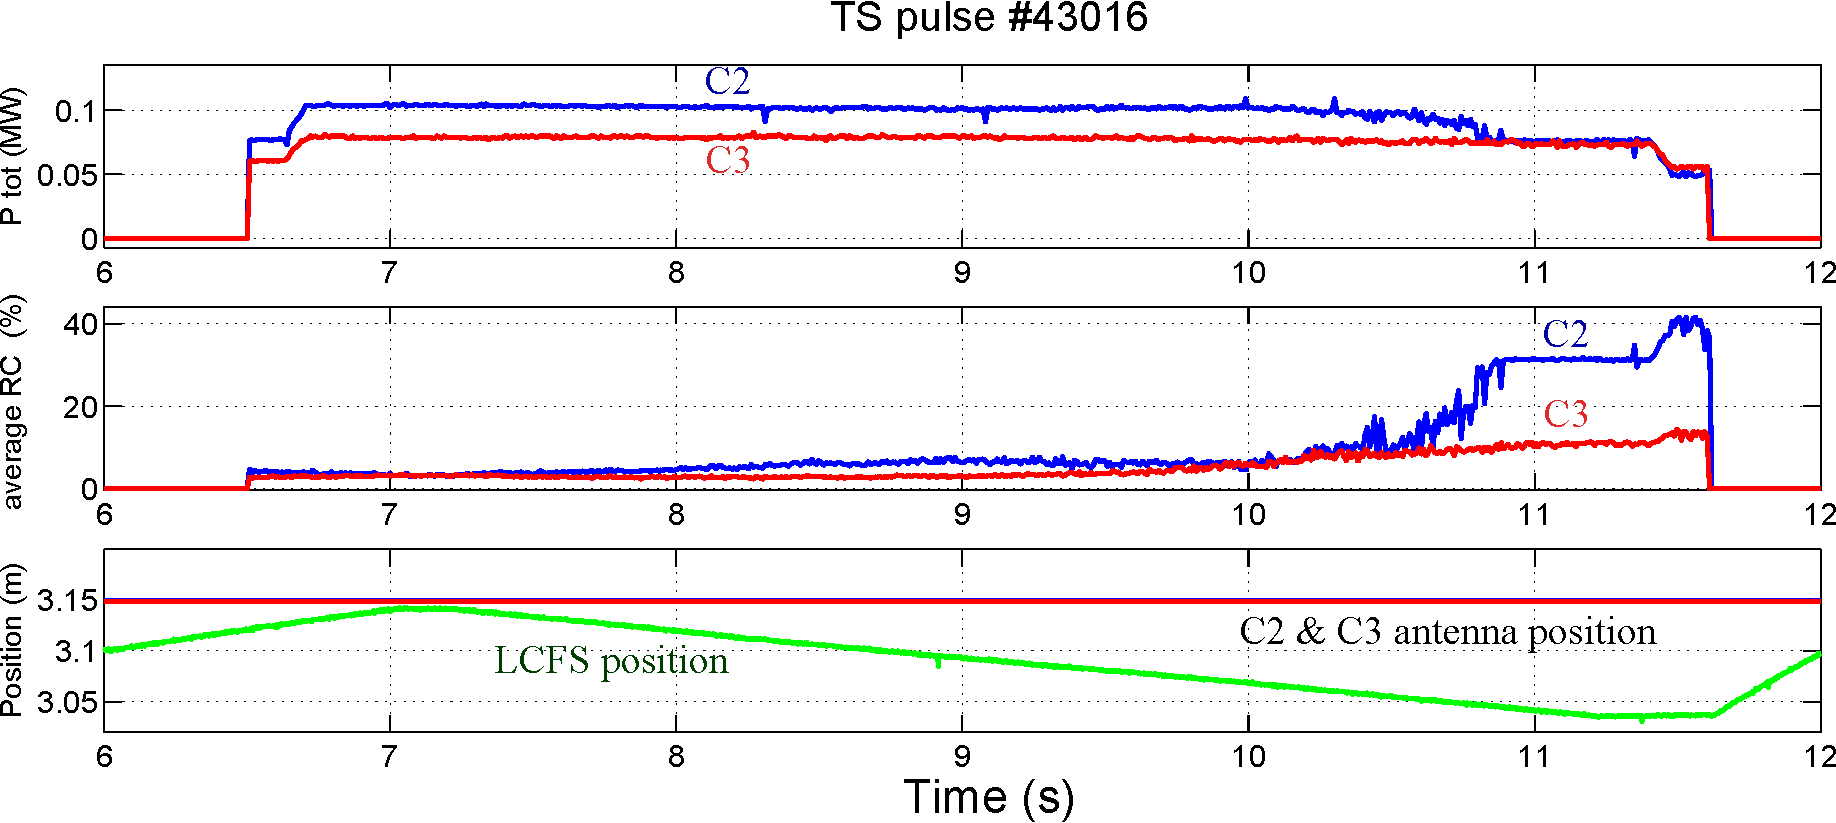
\includegraphics{figures/chap2/Tore_Supra/TS43016}
	\caption{Tore Supra pulse $\#43016$. Top: total power; middle: reflection coefficient; bottom: plasma LCFS and antenna positions.}
	\label{fig:TS43016}
\end{figure}

%Also shown are the poloidal cross sections of the plasma at the time of the RFA measurements at t = 7.05, 9.2 and 10.9 s (strictly speaking these are the poloidal cross sections for 42939 but I found very similar cross sections for all shots). The densities (as well as other RFA parameters like Jsat, Ti and Te) measured for different shots and fixed time are very similar because the plasma density is almost identical for all shots, the difference in the heating power between shots is very small and Ip is constant. The density e-folding increases slightly as the plasma moves from the APL during the shot, which could be explained by the enhancement of the particle transport on the LFS, as demonstrated earlier by the Jamie�s Mach probe measurements.

In ALOHA, the edge plasma is described with a linear electron density profile and no vacuum layer in front of the grill. RFA measurements have been used to estimate typical scrape-off thickness in front of the antennas\cite{kocan2008-1}. The connection lengths $L_{c,LH}$ in front of C2 and C3, corresponding to the distance between protruding side limiters, are known to be $40~\si{cm}$ and $60~\si{cm}$. Assuming that the ratio of the cross-field diffusion coefficient $D_\perp$ and the plasma acoustic velocity $c_s$ is constant in the SOL, and using scrape-off thickness defined as $\lambda_n=\frac{n_{e0}}{\nabla n_{e0}}=\sqrt{\frac{D_\perp L_c}{c_s}}$, one finds that $\lambda_{n,LH}=\sqrt{\frac{L_{c,RFA}}{L_{c,LH}}\lambda_{n,RFA}^2}$. 



% #################################################
% #################################################
% #################################################
\subsubsection{C2 antenna}
We present here some comparisons between experimental measurements and ALOHA on the Tore Supra C2 antenna. This antenna, installed in 1991, has been removed in 2009 and replaced by a new passive-active multi-junction antenna\cite{guilhem2009,guilhem2011}. The C2 antenna is made of 8 modules. Each module line is a 1-to-4 multi-junction (cf.~Fig~\ref{fig:geometry_TS_LHAntennas}). Permanent built-in phase shifters produce a $90^\circ$ phase difference between each output waveguides on a toroidal line, which produce a nominal peak parallel index of $n_{\parallel,0}=1.82$.

\begin{figure}[h]
	\centering
	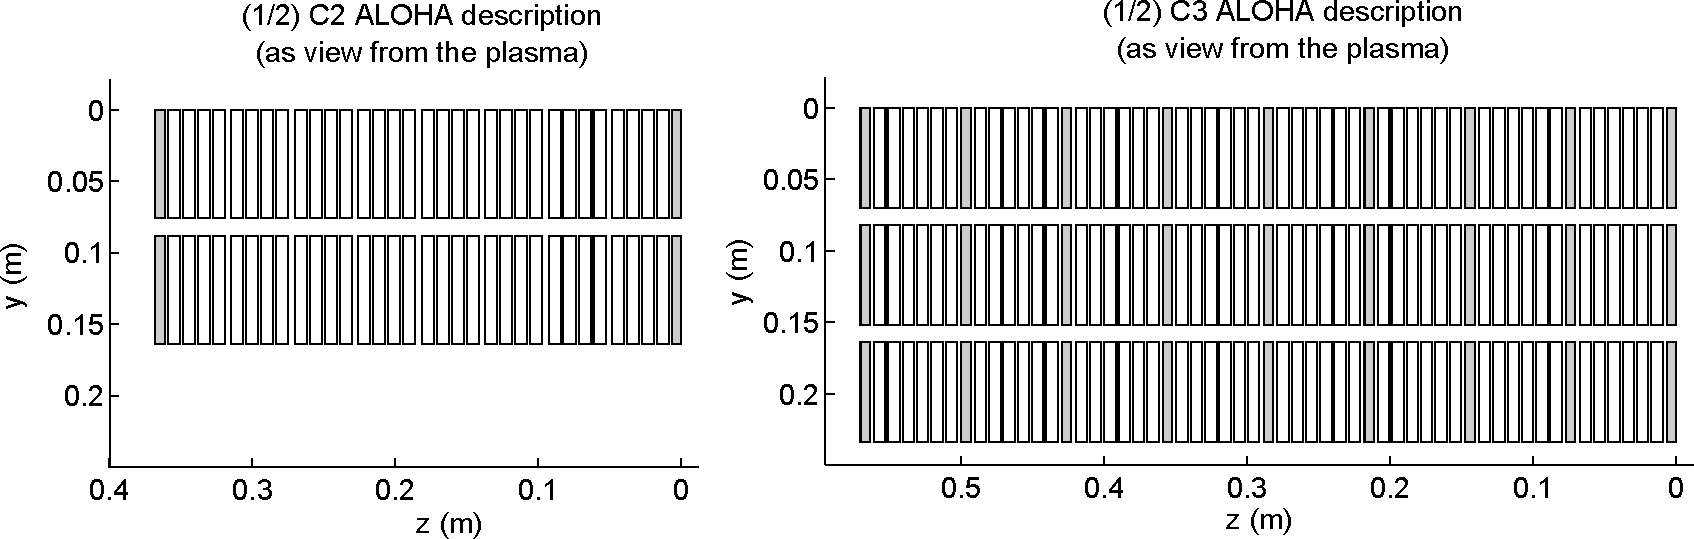
\includegraphics[width=1.0\textwidth]{figures/chap2/Tore_Supra/geometry_TS_LHAntennas}
	\caption{ALOHA description of the upper parts of C2 and C3 antennas . Grey parts symbolizes passive waveguides.}
	\label{fig:geometry_TS_LHAntennas}
\end{figure}

In Figure~\ref{fig:MarkI_mean_RC}, experimental reflection coefficients at different electron densities, measured during Tore Supra pulses \#43014-43016 for 5 upper modules of the C2 antenna are plotted. The density is measured with the nearest Langmuir probe placed at the center of the C2 antenna. Plain black line corresponds to the reflection coefficient calculated with ALOHA for different electron density values $n_{e0}$ at the mouth of the antenna for $\lambda_n=7$~mm. Dotted lines are for$\lambda_n=5$ and $10$~mm. For the C2 antenna, RFA measurements give $\lambda_n$ in $[3.3, 6.5]$~mm, which is in agreement with ALOHA results. 

\begin{figure}[h]
	\centering
	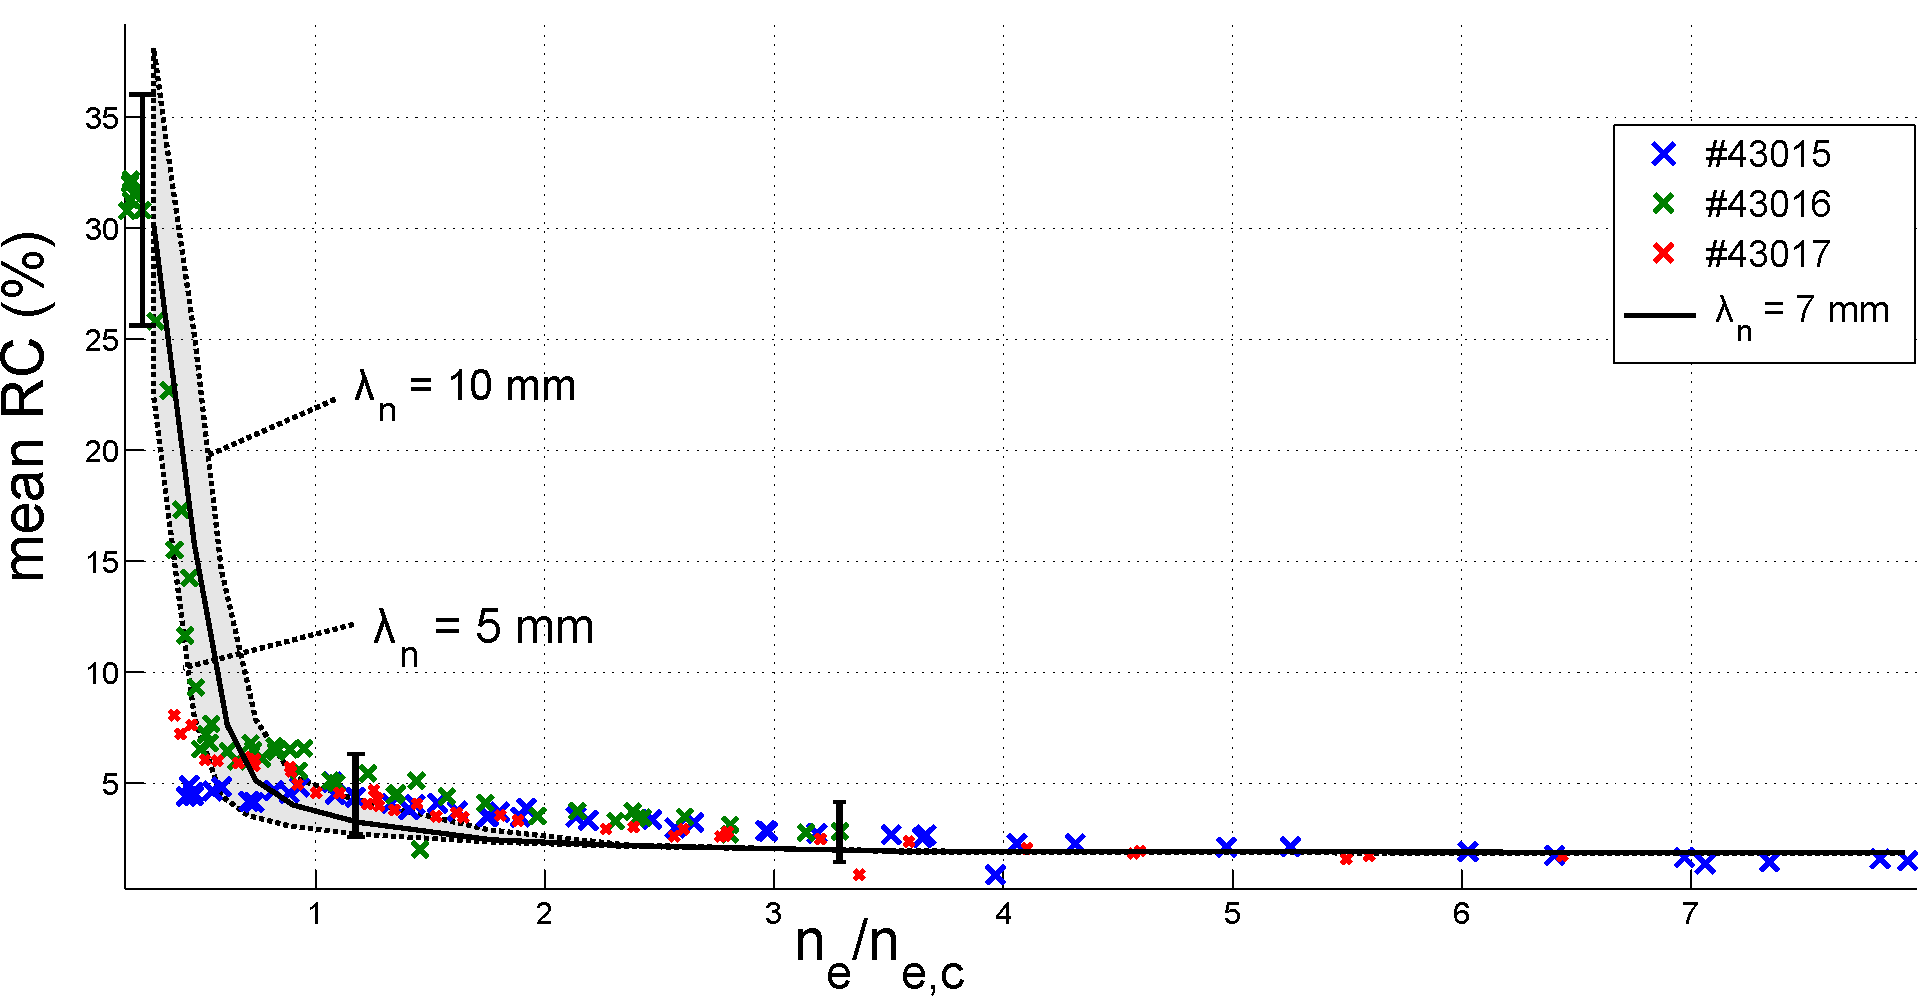
\includegraphics[width=0.95\textwidth]{figures/chap2/Tore_Supra/C2_mean_CR_modBas}
	\caption{Average reflection  coefficient (in percents) versus electron density (normalized to LH cut-off density) for C2 antennas. Measured reflection  coefficient are taken from TS pulses number 43014-43016. Black curve corresponds to a $2~mm$ scrape-off thickness ($\pm 1~mm$).}
	\label{fig:MarkI_mean_RC}
\end{figure}

% #################################################
% #################################################
% #################################################
\subsubsection{C3 antenna}
C3\sidenote{The antenna has been relabelled LH1 in WEST.} has been installed in 1999 and is also made of 8 modules. Each module is a 1-to-6 multi-junction (cf. Figure~\ref{fig:geometry_TS_LHAntennas}). Permanent built-in phase shifters produce a $90^\circ$ phase difference between each output waveguides on a toroidal line, which produce a nominal peak parallel index of $n_{\parallel,0}=2.02$.

In Figure~\ref{fig:MarkII_mean_RC}, experimental reflection coefficients at different electron densities, measured during Tore Supra pulses \#43014-43016 for the 4 first lower modules of the C3 antenna are plotted. The density is measured with the nearest Langmuir probe placed at the bottom of the C3 antenna. 

\begin{figure}[h]
	\centering
	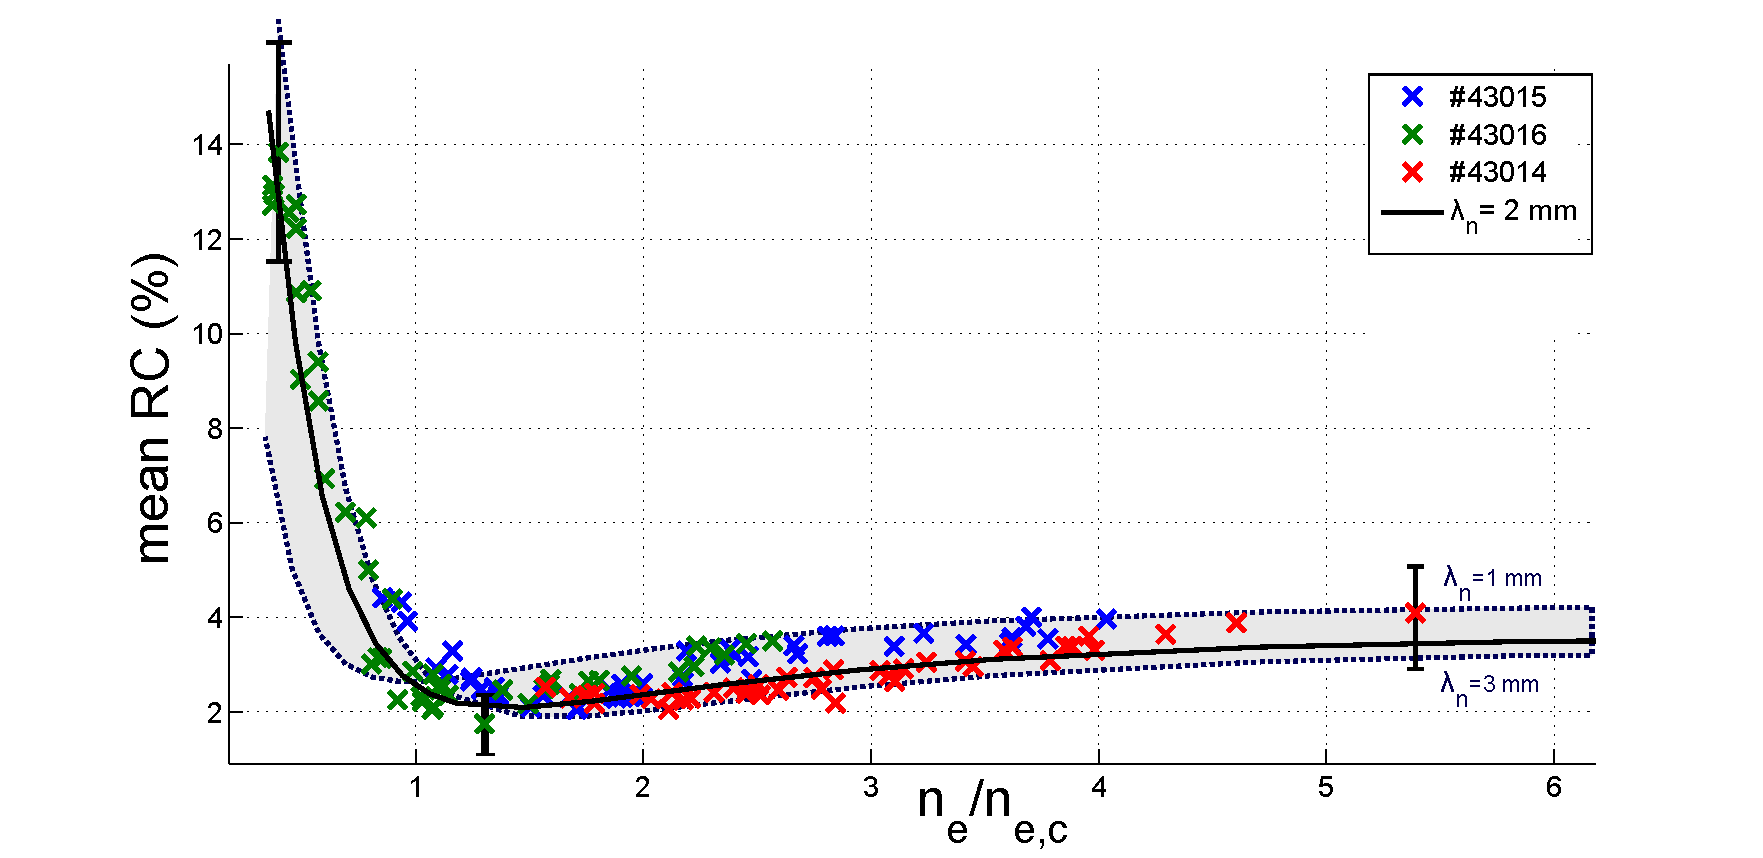
\includegraphics[width=0.95\textwidth]{figures/chap2/Tore_Supra/C3_mean_lowerMod}
	\caption{Average reflection  coefficient (in percents) versus electron density (normalized to LH cut-off density) for C3 antennas. Measured reflection  coefficient are taken from TS pulses number 43014-43016. Black curve corresponds to a $2~mm$ scrape-off thickness ($\pm 1~mm$).}
	\label{fig:MarkII_mean_RC}
\end{figure}




% ##################################################
\subsubsection{C4 antenna}
\todo{Figures Mélanie}

% ##################################################
\subsubsection{Summary of this section}

Experimental reflection coefficients at different electron densities, measured during Tore Supra pulses had been compared with the ALOHA code predictions. Results obtained with ALOHA are in good agreement with the experimental measurements for both Tore Supra antennas and shows that ALOHA is an efficient LH predictive tool. 

% ###################################################
% ###################################################
\subsection{Full-Wave Antenna Coupling}\label{sec:LHCD_FW_antena_coupling}
\marginnote{Part of this section are taken from paper \cite{hillairet2019}.}



%\subsection{Resonance Cone}
%Bellan and Porkolab PRL 34, 124, 1975.
%
%
%\subsection{Overview of parameters achieved and example of some systems}
%\subsubsection{LH Launchers main figures of merit}
%
%There are three important figures of merit to measure the efficiency and the performances of a LH launcher: 
%\begin{enumerate}
%	\item The first one is the k-space radiated power spectrum, generally characterized by its \emph{parallel power spectrum} $p(n_{\parallel})$ . This quantity represents the amount of power for each parallel index excited by the launcher. The relation between this power spectrum and the array excitation is related to the Fourier transform of the electromagnetic field at the plasma-antenna interface. 
%	
%	\item  The second one is the ratio of the reflected power (at the mouth or at the end of the launcher) to the input power, named the \emph{reflection coefficient} (sometime expressed in percent). 
%	$$RC = \frac{P_r}{P_i}$$
%	\item The third one is the \emph{directivity} of the launcher, which is the fraction of the power spectrum over its total power content. It can be viewed as the fraction of the power that goes toward one toroidal direction over the total coupled power. One can define the directivity as follow\footnote{Other definitions exist, essentially in order to ad a physical content to the directivity, in relation with the current drive efficiency evolution in the plasma. See for instance \sidecite{Litaudon1990a}.}
%	$$
%	D
%	= 
%	\frac{
%		\int_{n_{\parallel} >0} p(n_{\parallel}) dn_{\parallel} 
%	}{
%		\int_{n_{\parallel}} p(n_{\parallel}) dn_{\parallel} } 
%	$$
%\end{enumerate}
%
%Theoretically, if the $n_{\parallel}$ spectrum of an antenna is known, one can evaluate the reflection coefficient. However, since the wave field at the launcher aperture (and thus the launcher spectrum) depends on the plasma itself, numerical codes are required to make a self-consistent numerical evaluation of the coupling. Such codes are coupling codes.
%
%\subsection{LH systems and launchers performances}
%Mainly because of its relative simplicity, most of the LH launchers have been based on a "grill" configuration, as for example in the 1980' \sidecite{porkolab1984a, gormezano1986a, Stevens1988}.
%
%Typical grill launchers have a high reflection coefficient (of the order of 20 to 40\%) but directivity higher than 80\%. Since all the waveguides can be feed by independent RF sources, and thus independently phased, such launchers have a wide flexibility in terms of operational space (excited spectrum) which is of great interest for physics studies. However, since each waveguide is independently power fed, the complexity of the launcher grows enormously with the number of output waveguides, leading to cumbersome transmission systems for multi-megawatt power levels (Table \ref{tab:grillperformances}). 
%
%
%Multijunction launchers at the contrary have led to hundred of waveguides launchers (see Table \ref{tab:multijunctionperformances}). The complexity of the multijunction design and manufacturing is balanced by the a simpler transmission line system behind the launcher. Because of the self-matching property, the typical reflection coefficient of multijunction launchers is generally less than 10\%. However, the multiple back and forth of the waves leads to an increase of the peak electric field in secondary waveguides. Moreover, since the phase shift is created by the built-in phase shifter inside the launcher, the flexibility of phase configuration is reduced in comparison to classic grill launchers. 
%
%
%The PAM concept tested in FTU and in the Tore Supra tokamak showed that reflected power lower than 5\% (i.e. high coupling efficiency) and continuous operations could be combined (cf. Figure \ref{fig:ts45472c4ir}) during long pulse operations. 
%
%
%
%\subsection{ITER System}
%
%Although not part of the ITER initially planned procurement phase, a conceptual design of a 20~MW/CW 5~GHz LHCD system has been proposed for the second mission of ITER, i.e. Q=5 steady state target \sidecite{hoang2009}. In ITER, the parallel index of the launched waves $n_{\parallel 0}$ ~ 2.0 has been selected as a trade-off between the current drive efficiency, the wave accessibility and the location of power deposition, all of which depend upon the plasma conditions. Depending of the plasma scenarios (steady-state, hybrid, ramp-up, etc.), the additional current driven by LHCD would range between 0.42 MA (steady-state) up to more than 3.0 MA (ramp-up) \sidecite{decker2011}. In any case, these values confirm that for steady state scenarios, a substantial bootstrap current is required \sidecite{jacquinot1999}. The average current drive efficiency, which is the figure of merit of the LHCD, has been calculated to be $\eta \equiv 0.2 \times 10^{20} A m^{-2} W^{-1}$, similar to the ones measured in present days tokamaks \sidecite{jacquinot1999}. This value can be compared to other additional current drive scheme, such as NBI or ECCD. 
%
%In addition, LHCD-assisted start-up could reduce the flux consumption during current ramp-up, resulting in a longer flat top or burn time. An early application of 20 MW LHCD during the plasma current ramp-up phase of the ITER reference scenario 2 is effective to reduce the flux consumption. An expected saved flux of 43Wb is equivalent to about 500 s of additional burn duration \sidecite{hoang2009}.
%
